\documentclass[10pt, a4paper]{article}

% ----- packages -----
\usepackage{amsmath} % AMS mathematical facilities for LaTeX
\usepackage{enumitem} % Control layout of itemize, enumerate, description
\usepackage{fancyhdr} % Extensive control of page headers and footers in LaTeX2
\usepackage{geometry} % Flexible and complete interface to document dimensions
\usepackage{graphicx} % Enhanced support for graphics
\usepackage{hyperref} % Extensive support for hypertext in LaTeX
\usepackage{parskip} % Layout with zero \parindent, non-zero \parskip
\usepackage{titlesec} % Select alternative section titles
\usepackage{multirow} % Create tabular cells spanning multiple rows

% ----- custom commands -----
% simple interest formulas
\newcommand{\Sif}{$C_{n} = C_{0} \cdot (1 + i \cdot n)$}
\newcommand{\SifRateim}{$i_{m} = \dfrac{i}{m}$}
\newcommand{\SifSolveCo}{$C_{0} = \dfrac{C_{n}}{1 + i \cdot n}$}
\newcommand{\SifSolvei}{$i = \dfrac{\frac{C_{n}}{C_{0}} - 1}{n}$}
\newcommand{\SifSolven}{$n = \dfrac{\frac{C_{n}}{C_{0}} - 1}{i}$}
% compound interest formulas
\newcommand{\Cif}{$C_{n} = C_{0} \cdot (1 + i)^{n}$}
\newcommand{\CifRateim}{$i_{m} = (1 + i)^{1 / m} - 1$}
\newcommand{\CifRatei}{$i = (i_{m} + 1)^{m} - 1$}
\newcommand{\CifSolveCo}{$C_{0} = \dfrac{C_{n}}{(1 + i)^{n}}$}
\newcommand{\CifSolvei}{$i = \left(\dfrac{C_{n}}{C_{0}}\right)^{1 / n} - 1$}
\newcommand{\CifSolven}{$n = \dfrac{\log{\left(\frac{C_{n}}{C_{0}}\right)}}{\log{(1 + i)}}$}
% simple discount formulas
\newcommand{\Sdf}{$C_{0} = C_{n} (1 - d \cdot n)$}
\newcommand{\SdfRatedm}{$d_{m} = \dfrac{d}{m}$}
\newcommand{\Sdfr}{\textbf{Rational} \quad $C_0 = \dfrac{C_{n}}{1 + i \cdot n}$}
% compound discount formula
\newcommand{\Cdf}{$C_{0} = C_{n} \cdot (1 - d)^{n}$}
% temporal unitary rent formulas
\newcommand{\TurfPoa}{$a_{n \rceil i} = \dfrac{1 - (1 + i)^{-n}}{i}$}
\newcommand{\TurfPos}{$S_{n \rceil i} = a_{n \rceil i} \cdot (1 + i)^{n}$}
\newcommand{\TurfPra}{$\ddot{a}_{n \rceil i} = (1 + i) \cdot a_{n \rceil i}$}
\newcommand{\TurfPrs}{$\ddot{S}_{n \rceil i} = (1 + i) \cdot s_{n \rceil i}$}
% perpetual unitary rent formulas
\newcommand{\PurfPoa}{$a_{\infty \rceil i} = \dfrac{1}{i}$}
\newcommand{\PurfPra}{$\ddot{a}_{\infty \rceil i} = (1 + i) \cdot a_{\infty \rceil i}$}
% temporal geometric rent formulas
\newcommand{\TgrfPoA}{$A(C;q)_{n \rceil i} =
	\begin{cases}
		C \cdot \dfrac{1 - \left( \dfrac{q}{1 + i} \right)^n}{1 + i - q} & \mathrm{si} \quad q \neq 1 + i \\
		C \cdot \dfrac{n}{1 + i}                                         & \mathrm{si} \quad q = 1 + i
	\end{cases}$}
\newcommand{\TgrfPoS}{$S(C;q)_{n \rceil i} = A(C;q)_{n \rceil i} \cdot (1 + i)^n$}
\newcommand{\TgrfPrA}{$\ddot{A}(C;q)_{n \rceil i} = (1 + i) \cdot A(C;q)_{n \rceil i}$}
\newcommand{\TgrfPrS}{$\ddot{S}(C;q)_{n \rceil i} = (1 + i) \cdot S(C;q)_{n \rceil i}$}
% perpetual geometric rent formulas
\newcommand{\PgrfPoA}{$A(C;q)_{\infty \rceil i} =
	\begin{cases}
		C \cdot \dfrac{1}{1 + i - q} & \mathrm{si} \quad q < 1 + i    \\
		\mathrm{Infinito}            & \mathrm{si} \quad q \geq 1 + i
	\end{cases}$}
\newcommand{\PgrfPrA}{$\ddot{A}(C;q)_{\infty \rceil i} = (1 + i) \cdot A(C;q)_{\infty \rceil i}$}
% constant
\newcommand{\Const}{Constante}
% loan french type
\newcommand{\Lfta}{$a = \dfrac{C_{0}}{a_{n \rceil i}}$}
\newcommand{\LftA}{$A_{s} = A_{1} \cdot (1 + i)^{s - 1}$}
\newcommand{\LftC}{$C_{0} = A_{1} \cdot S_{n \rceil i}$}
\newcommand{\LftCRec}{$C_{s} = C_{s - 1} \cdot (1 + i) - a$}
\newcommand{\LftCPro}{$C_{s} = a \cdot a_{n - s \rceil i}$}
\newcommand{\LftCRet}{$C_{s} = C_{0} \cdot (1 + i)^{s} - a \cdot S_{s \rceil i}$}
% loan american type
\newcommand{\Latas}{$a_{s} = I_{s} = C_{0} \cdot i_{s} \quad \mathrm{si} \quad s \neq n$}
\newcommand{\Latan}{$a_{n} = I_{n} + C_{0} = C_{0} \cdot i_{s} + C_{0} \quad \mathrm{si} \quad s = n$}
\newcommand{\LatAs}{$A_{s} = 0 \quad \mathrm{si} \quad s \neq n$}
\newcommand{\LatAn}{$A_{n} = C_{0} \quad \mathrm{si} \quad s = n$}
\newcommand{\LatCs}{$C_{s} = C_{0} \quad \mathrm{si} \quad s \neq n$}
\newcommand{\LatCn}{$C_{n} = 0 \quad \mathrm{si} \quad s = n$}
% loan italian type
\newcommand{\Lita}{$a_{s + 1} = a_{s} - i \cdot A$}
\newcommand{\LitI}{$I_{s + 1} = I_{s} - i \cdot A$}
\newcommand{\LitA}{$A = \dfrac{C_{0}}{n}$}
\newcommand{\LitCRec}{$C_{s} = C_{s - 1} - A$}
\newcommand{\LitCPro}{$C_{s} = C_{n - s} \cdot A$}
\newcommand{\LitCRet}{$C_{s} = C_{0} - s \cdot A$}
% loan geometrical type
\newcommand{\Lgta}{$a = \dfrac{C_{0}}{A(1;q)_{n \rceil i}}$}
\newcommand{\LgtCRec}{$C_{s} = C_{s - 1} \cdot (1 + i) - a \cdot q^{s - 1}$}
\newcommand{\LgtCPro}{$C_{s} = A(a \cdot q^{s};q)_{n - s \rceil i}$}
\newcommand{\LgtCRet}{$C_{s} = C_{0} \cdot (1 + i)^{s} - S(a;q)_{s \rceil i}$}
% vertical text
\newcommand{\vtext}[1]{
	\rotatebox[origin=c]{90}{#1}
}

% ----- page customization -----
\geometry{margin=1cm} % margins config
\pagenumbering{gobble} % remove page numeration
\setlength{\parskip}{0cm} % paragraph spacing
% title spacing
\titlespacing{\section}{0pt}{2ex}{1ex}

% ----- footer -----
\pagestyle{fancy}
\renewcommand{\headrulewidth}{0pt}
\cfoot{\href{https://github.com/marcelomijas/financial-math-cheatsheet}{\normalfont \footnotesize FM-25.01-EN - github.com/marcelomijas/financial-math-cheatsheet - CC-BY-4.0 license}}
\setlength{\footskip}{12pt}

% ----- document -----
\begin{document}
	\begin{center}
		\textbf{\LARGE \href{https://github.com/marcelomijas/financial-math-cheatsheet}{Financial Mathematics Cheat Sheet}}
		
		{\footnotesize By Marcelo Moreno - Universidad Rey Juan Carlos}
	\end{center}

	\section*{Capitalization and discount}

	\begin{center}
		\renewcommand{\arraystretch}{2.5}
		\begin{tabular}{|c|cc|cc|}
			\hline
			                                           &    \multicolumn{2}{c|}{\textbf{Capitalization}}     &       \multicolumn{2}{c|}{\textbf{Discount}}        \\ \hline
			 \multirow{2}{*}{\vtext{\textbf{Simple}}}  & \multirow{2}{*}{\Sif} & \multirow{2}{*}{\SifRateim} & \Sdf &                  \SdfRatedm                  \\
			                                           &                       &                             &         \multicolumn{2}{c|}{\textbf{\Sdfr}}         \\ \hline
			\multirow{2}{*}{\vtext{\textbf{Compound}}} & \multirow{2}{*}{\Cif} &         \CifRateim          & \multicolumn{2}{c|}{\multirow{2}{*}{\textbf{\Cdf}}} \\
			                                           &                       &          \CifRatei          &      &                                              \\ \hline
		\end{tabular}
	\end{center}
	
	\vspace*{0.5cm}
		
	Notes: $C_{n}$ capital in $t = n$, $C_{0}$ capital in $t = 0$, $n$ periods, $m$ subperiods, $i$ interest rate, $d$ discount rate. There is also the so-called \textbf{fractional capitalization}, $i_{m} = \frac{j(m)}{m}$, where $j(m)$ is the nominal interest rate payable per $m$.
	
	\section*{Clearing interest formulas}
		
	\begin{center}
		\renewcommand{\arraystretch}{2.4}
		\begin{tabular}{|c|c|}
			\hline
			\textbf{Simple interest formulas} & \textbf{Compound interest formulas} \\ \hline
			              \Sif                &                \Cif                 \\ \hline
			           \SifSolveCo            &             \CifSolveCo             \\ \hline
			           \SifSolvei             &             \CifSolvei              \\ \hline
			           \SifSolven             &             \CifSolven              \\ \hline
		\end{tabular}
	\end{center}
		
	\section*{Series}
	
	\begin{center}
		\renewcommand{\arraystretch}{2.6}
		\begin{tabular}{|c|c|c|c|}
			\hline
			                                            &                                       & \textbf{Unitary} & \textbf{Variable in geometric progression} \\ \hline
			\multirow{4}{*}{\vtext{\textbf{Temporal}}}  & \multirow{2}{*}{\textbf{Postpayable}} &     \TurfPoa     &                  \TgrfPoA                  \\
			                                            &                                       &     \TurfPos     &                  \TgrfPoS                  \\ \cline{2-4}
			                                            & \multirow{2}{*}{\textbf{Prepayable}}  &     \TurfPra     &                  \TgrfPrA                  \\
			                                            &                                       &     \TurfPrs     &                  \TgrfPrS                  \\ \hline
			\multirow{2}{*}{\vtext{\textbf{Perpetual}}} &         \textbf{Postpayable}          &     \PurfPoa     &                  \PgrfPoA                  \\ \cline{2-4}
			                                            &          \textbf{Prepayable}          &     \PurfPra     &                  \PgrfPrA                  \\ \hline
		\end{tabular}
	\end{center}
	
	\vspace*{0.5cm}
	
	Notes:
	\begin{itemize}[leftmargin=*]
		\item[] $q =$ factor.
		\item[] \textbf{Present discounted value}, example, $V_{0} = C \cdot a_{n \rceil i}$
		\item[] \textbf{Final capitalized value}, example, $V_{n} = C \cdot S_{n \rceil i}$
	\end{itemize}
	
	\newpage
	
	\section*{Amortization table}
	
	\begin{center}
		\renewcommand{\arraystretch}{2}
		\scalebox{0.90}{
		\begin{tabular}{|c|c|c|c|c|c|c|}
			\hline
			\multirow{2}{*}{\textbf{Period}} & \textbf{Interest} & \textbf{Amortization} &        \textbf{Interest}        &  \textbf{Amortization}  & \multirow{2}{*}{\textbf{Living capital}} &     \multirow{2}{*}{\textbf{Amortized capital}}     \\
			                                 &   \textbf{rate}   &     \textbf{term}     &        \textbf{payment}         &    \textbf{payment}     &                                          &                                                     \\ \hline
			               0                 &         -         &           -           &                -                &            -            &                 $C_{0}$                  &                          -                          \\ \hline
			            $t_{1}$              &      $i_{1}$      &        $a_{1}$        &   $I_{1} = C_{0} \cdot i_{1}$   & $A_{1} = a_{1} - I_{1}$ &         $C_{1} = C_{0} - A_{1}$          &               $M_{1} = C_{0} - C_{1}$               \\ \hline
			            $t_{2}$              &      $i_{2}$      &        $a_{2}$        &   $I_{2} = C_{1} \cdot i_{2}$   & $A_{2} = a_{2} - I_{2}$ &         $C_{2} = C_{1} - A_{2}$          &               $M_{2} = C_{1} - C_{2}$               \\ \hline
			            $\cdots$             &     $\cdots$      &       $\cdots$        &            $\cdots$             &        $\cdots$         &                 $\cdots$                 &                      $\cdots$                       \\ \hline
			            $t_{s}$              &      $i_{s}$      &        $a_{s}$        & $I_{s} = C_{s - 1} \cdot i_{s}$ & $A_{s} = a_{s} - I_{s}$ &       $C_{s} = C_{s - 1} - A_{s}$        &             $M_{s} = C_{s - 1} - C_{s}$             \\ \hline
			            $\cdots$             &     $\cdots$      &       $\cdots$        &            $\cdots$             &        $\cdots$         &                 $\cdots$                 &                      $\cdots$                       \\ \hline
			            $\cdots$             &     $\cdots$      &       $\cdots$        &            $\cdots$             &        $\cdots$         &                 $\cdots$                 &                      $\cdots$                       \\ \hline
			            $t_{n}$              &      $i_{n}$      &        $a_{n}$        & $I_{n} = C_{n - 1} \cdot i_{n}$ & $A_{n} = a_{n} - I_{n}$ &     $C_{n} = C_{n - 1} - A_{n} = 0$      & $M_{n} = C_{0} - C_{n} = M_{n - 1} + A_{n} = C_{0}$ \\ \hline
		\end{tabular}
		}
	\end{center}
	
	\section*{Loans}
	
	\begin{center}
		\renewcommand{\arraystretch}{3}
		\scalebox{0.90}{
		\begin{tabular}{|cc|c|c|c|c|}
			\hline
			                               &                         & \multirow{2}{*}{\textbf{French}} & \multirow{2}{*}{\textbf{American}} & \multirow{2}{*}{\textbf{Italian}} & \textbf{Geometric progression} \\
			                               &                         &                                  &                                    &                                   &         \textbf{terms}         \\ \hline
			\multicolumn{2}{|c|}{$i$}                                &              \Const              &                 -                  &                 -                 &               -                \\ \hline
			\multicolumn{2}{|c|}{\multirow{2}{*}{\textbf{$a$}}}      &             \Const;              &               \Latas               &      \multirow{2}{*}{\Lita}       &     \multirow{2}{*}{\Lgta}     \\
			                               &                         &              \Lfta               &               \Latan               &                                   &                                \\ \hline
			\multicolumn{2}{|c|}{$I$}                                &                -                 &                 -                  &               \LitI               &               -                \\ \hline
			\multicolumn{2}{|c|}{\multirow{2}{*}{\textbf{$A$}}}      &      \multirow{2}{*}{\LftA}      &               \LatAs               &              \Const;              &       \multirow{2}{*}{-}       \\
			                               &                         &                                  &               \LatAn               &               \LitA               &                                \\ \hline
			\multicolumn{2}{|c|}{\multirow{2}{*}{\textbf{$C$}}}      &              \LftC               &               \LatCs               &        \multirow{2}{*}{-}         &       \multirow{2}{*}{-}       \\
			                               &                         &                                  &               \LatCn               &                                   &                                \\ \hline
			  \vtext{\textbf{Recursive}}   & \vtext{\textbf{method}} &             \LftCRec             &                 -                  &             \LitCRec              &            \LgtCRec            \\ \hline
			 \vtext{\textbf{Prospective}}  & \vtext{\textbf{method}} &             \LftCPro             &                 -                  &             \LitCPro              &            \LgtCPro            \\ \hline
			\vtext{\textbf{Retrospective}} & \vtext{\textbf{method}} &             \LftCRet             &                 -                  &             \LitCRet              &            \LgtCRet            \\ \hline
		\end{tabular}
		}
	\end{center}
	
	\newpage
	
	\section*{Graphical analysis of loans}
	
	Suppose a loan with principal $C_{0} = 10.000$ at an interest rate $i = 10\%$ ending at $n = 12$ in which an amount is paid in each period that will depend on the type of loan.

	\textbf{French loan}: constant interest rate, all amortization terms are constant, amortization payments vary in geometric progression of factor $(1 + i)$:
	
	\begin{center}
		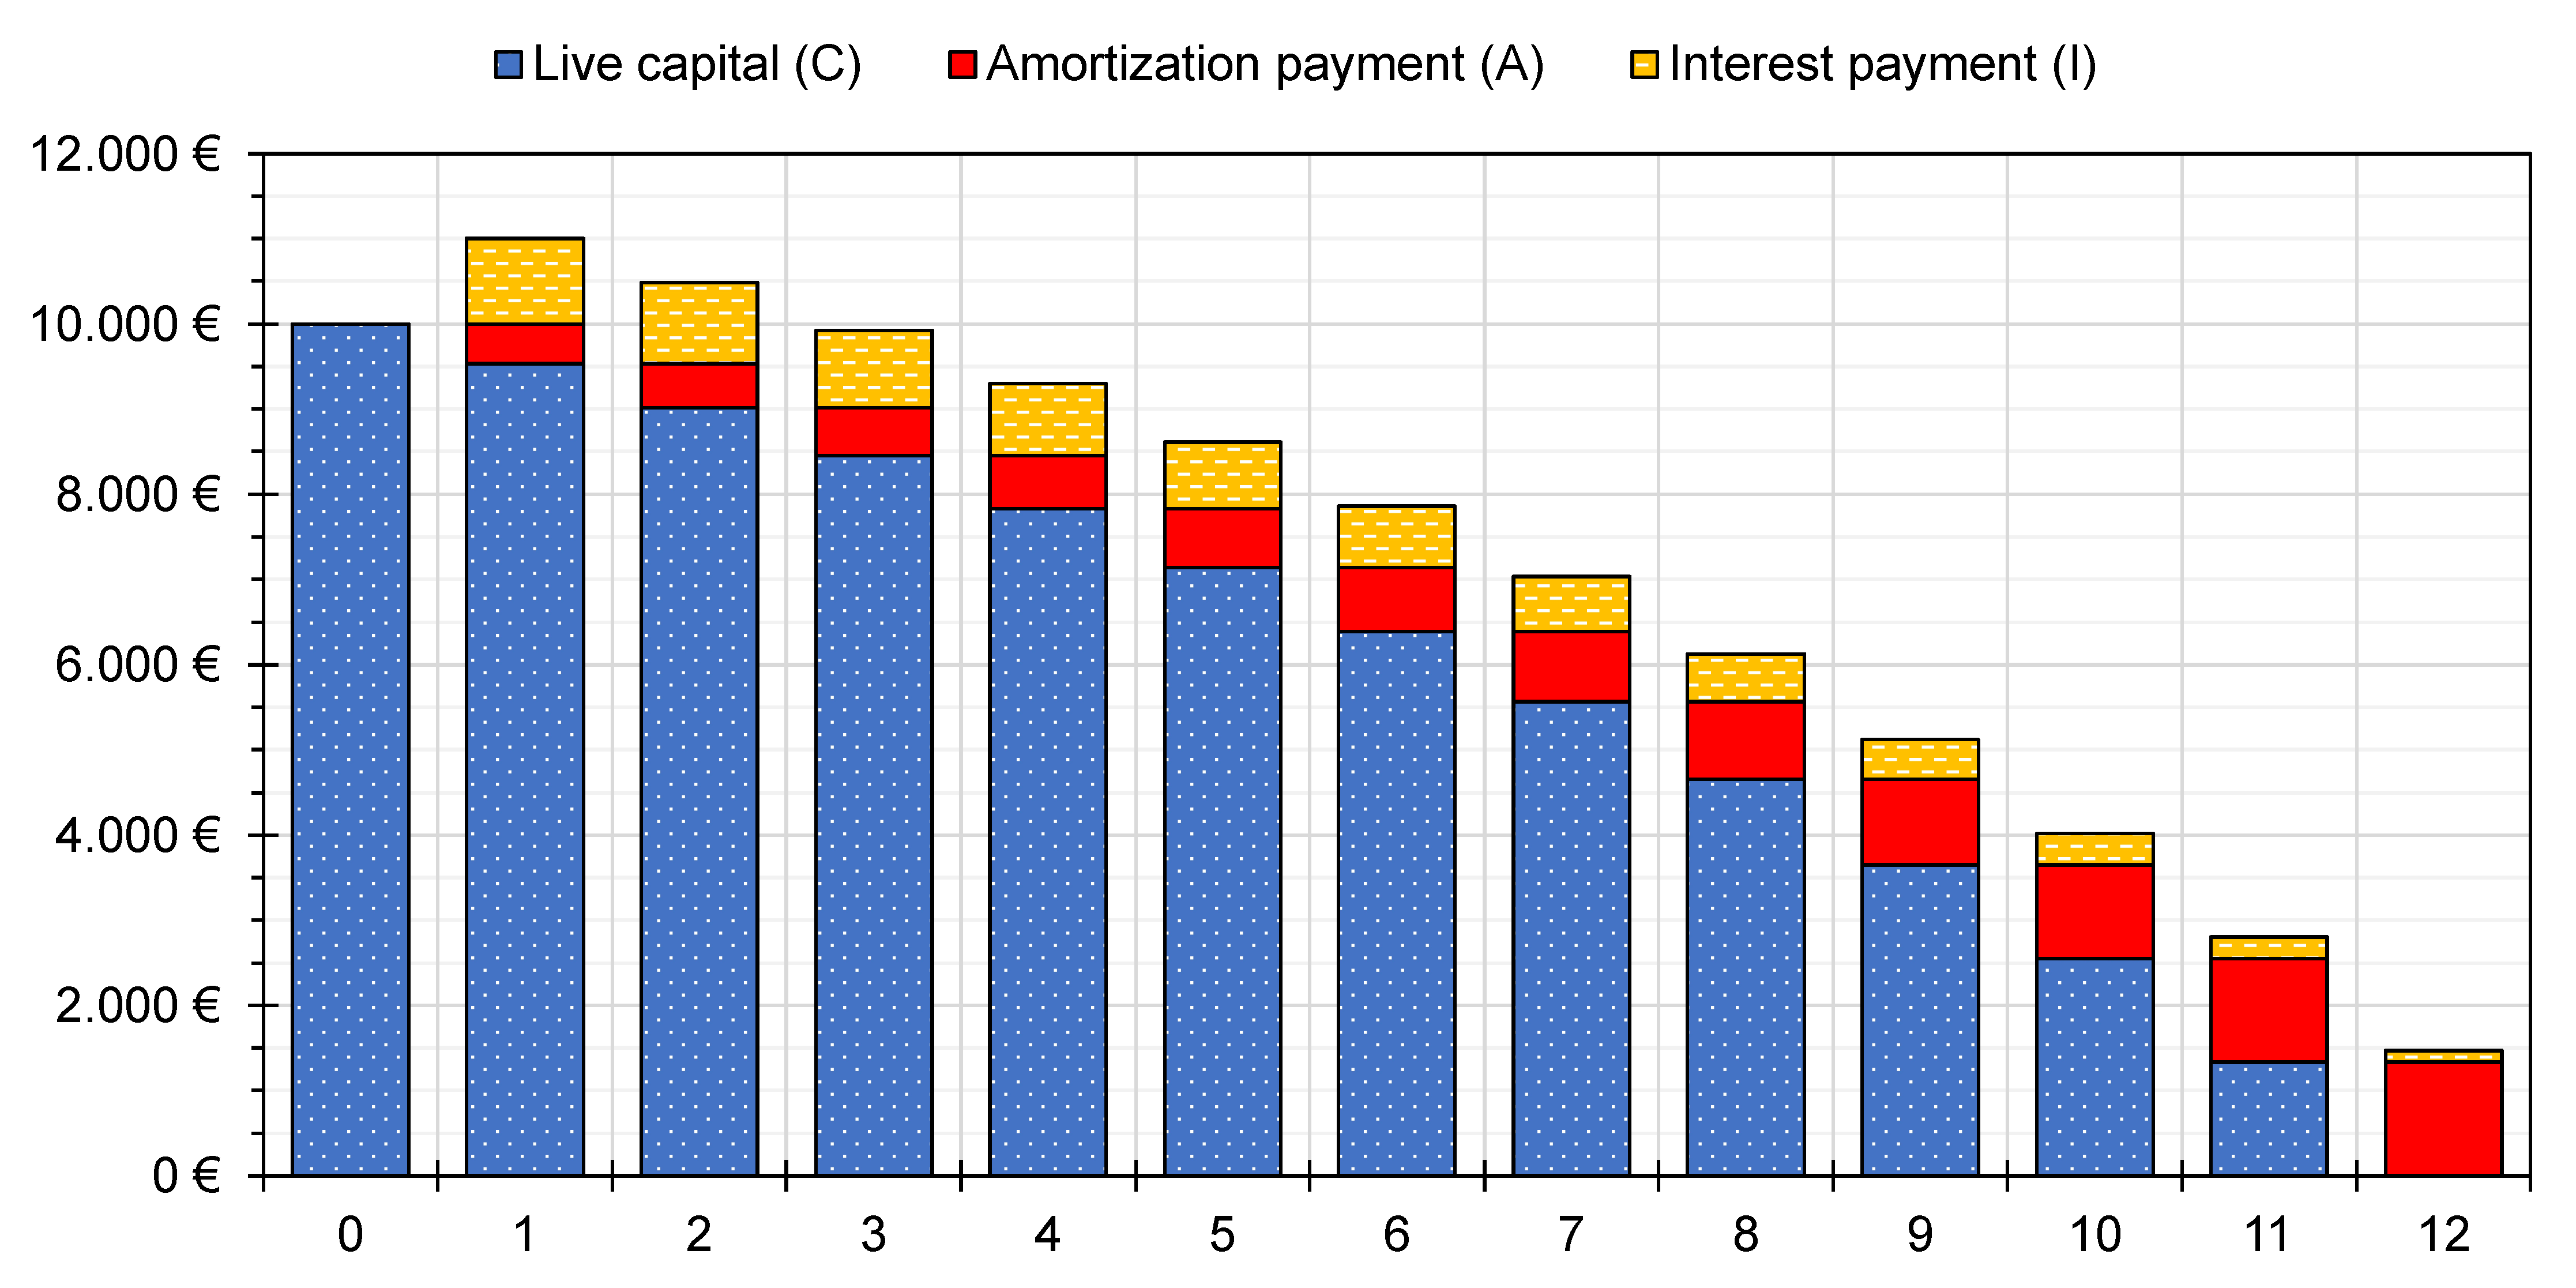
\includegraphics[width=11cm]{figures/french-en.pdf}
	\end{center}
		
	\textbf{American loan}: the debtor only pays interest at the end of each period except in the last, in which he also pays the nominal amount of the loan; the payments are only interest, the live capital does not vary until the last period.
	
	\begin{center}
		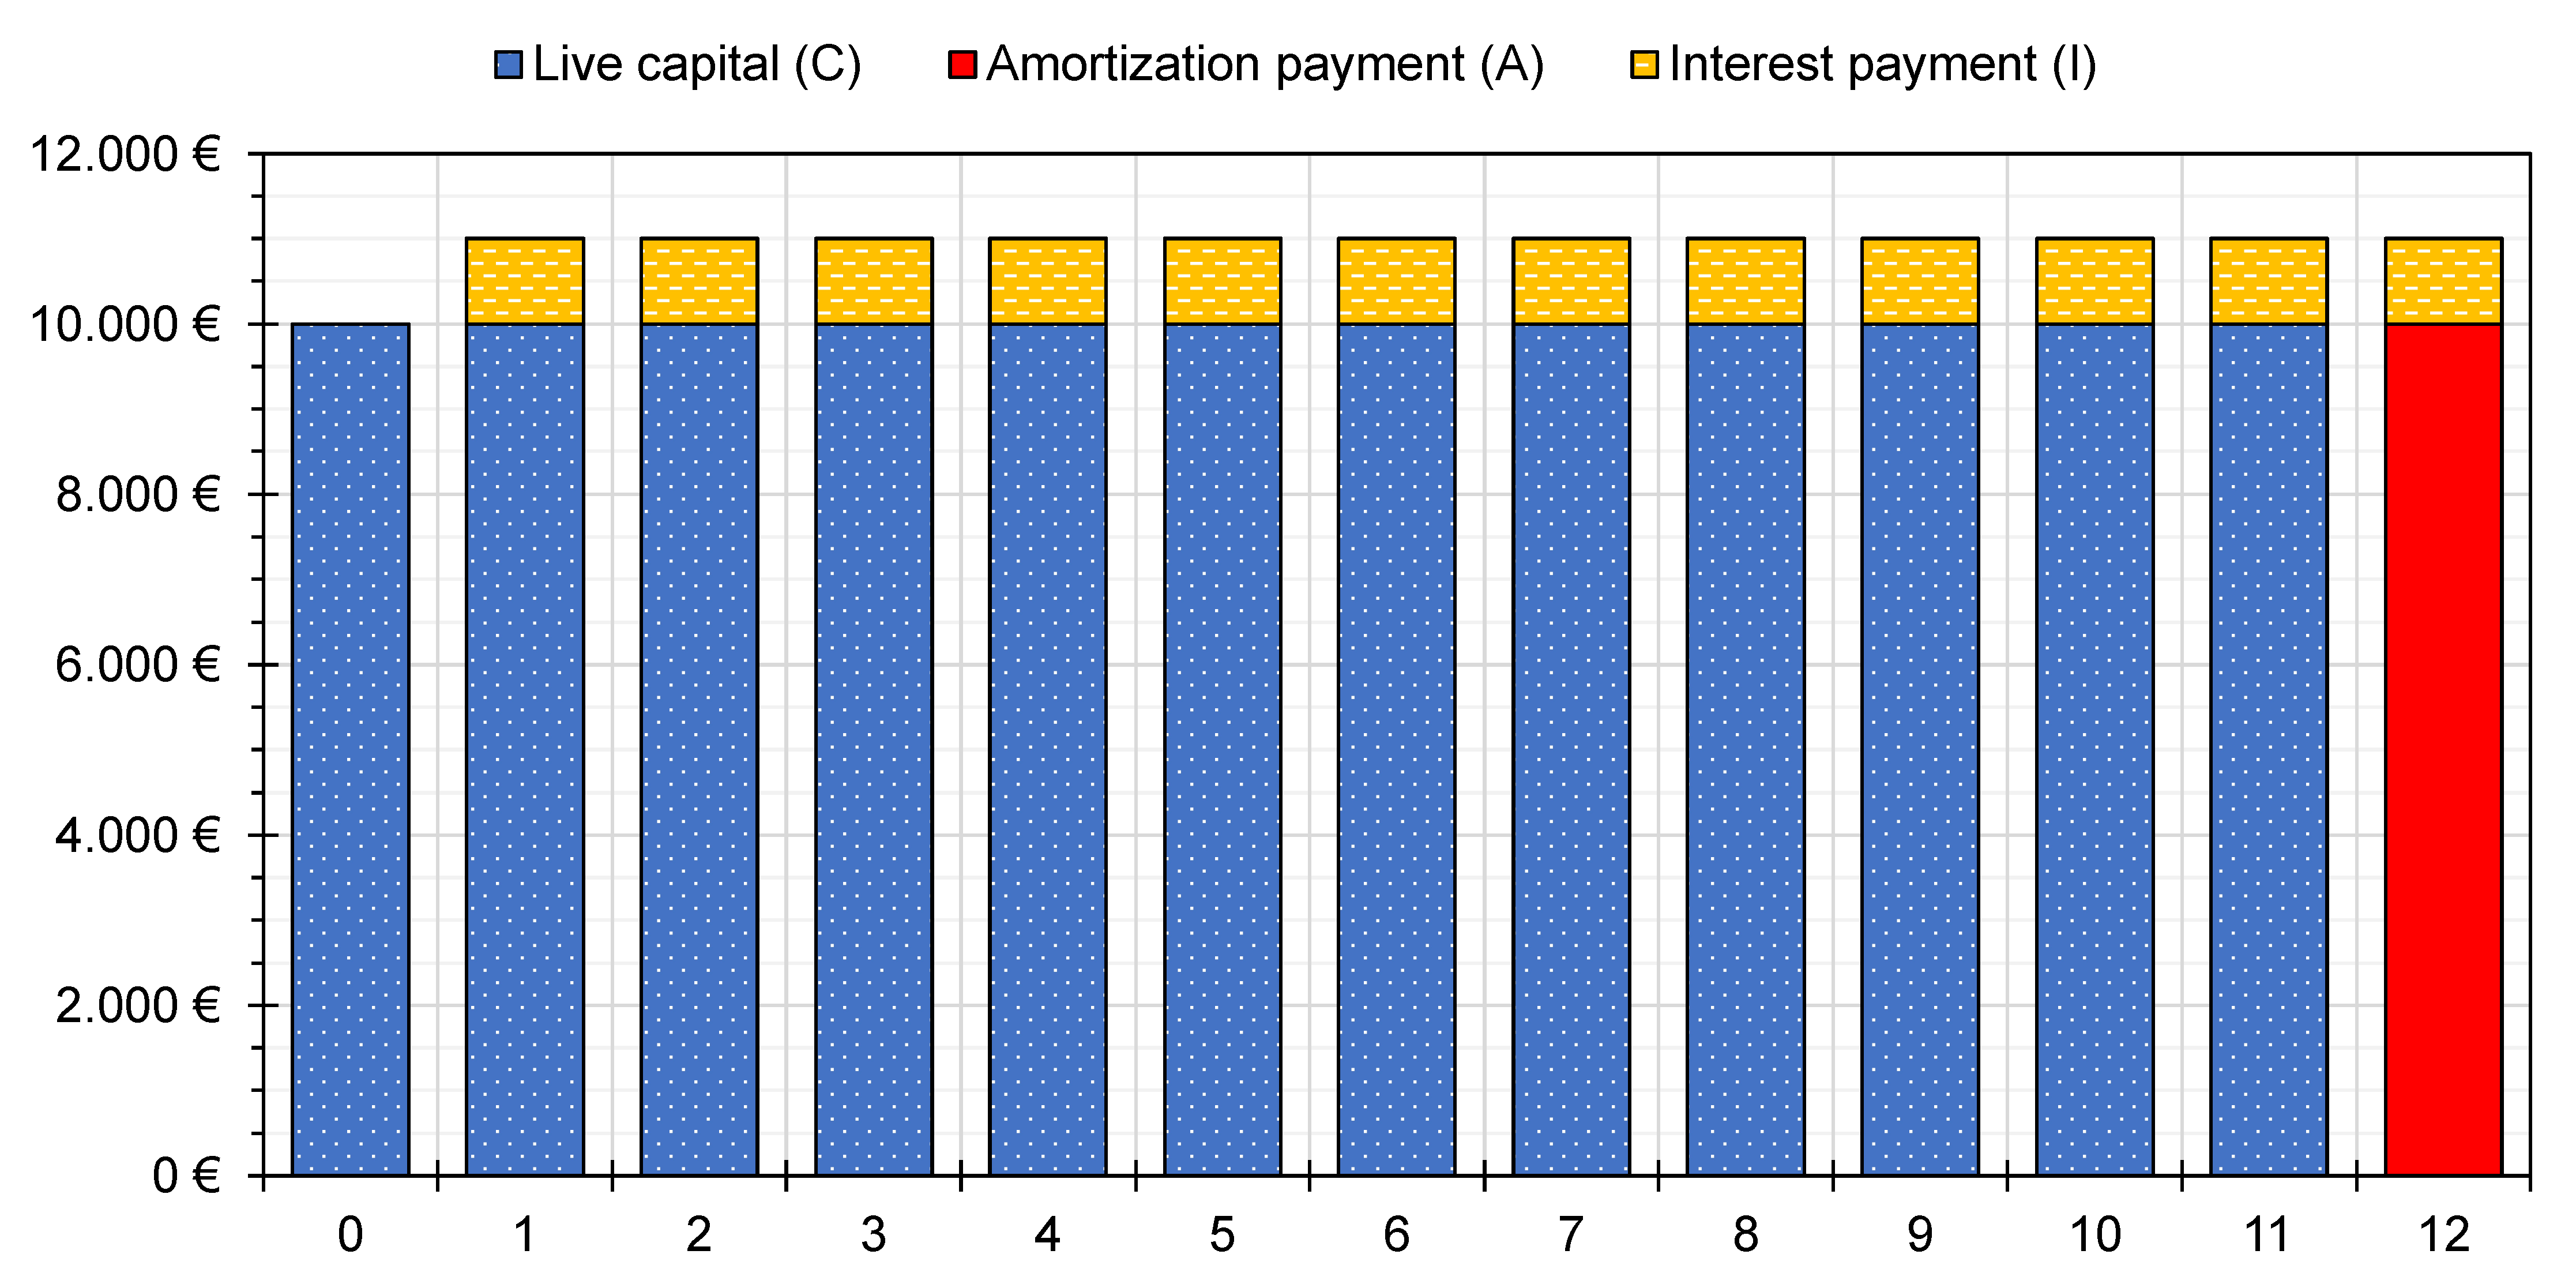
\includegraphics[width=11cm]{figures/american-en.pdf}
	\end{center}
	
	\textbf{Italian loan}: constant amortization payments, amortization terms and interest payments decrease in arithmetic progression ($-i \cdot A$).	
	
	\begin{center}
		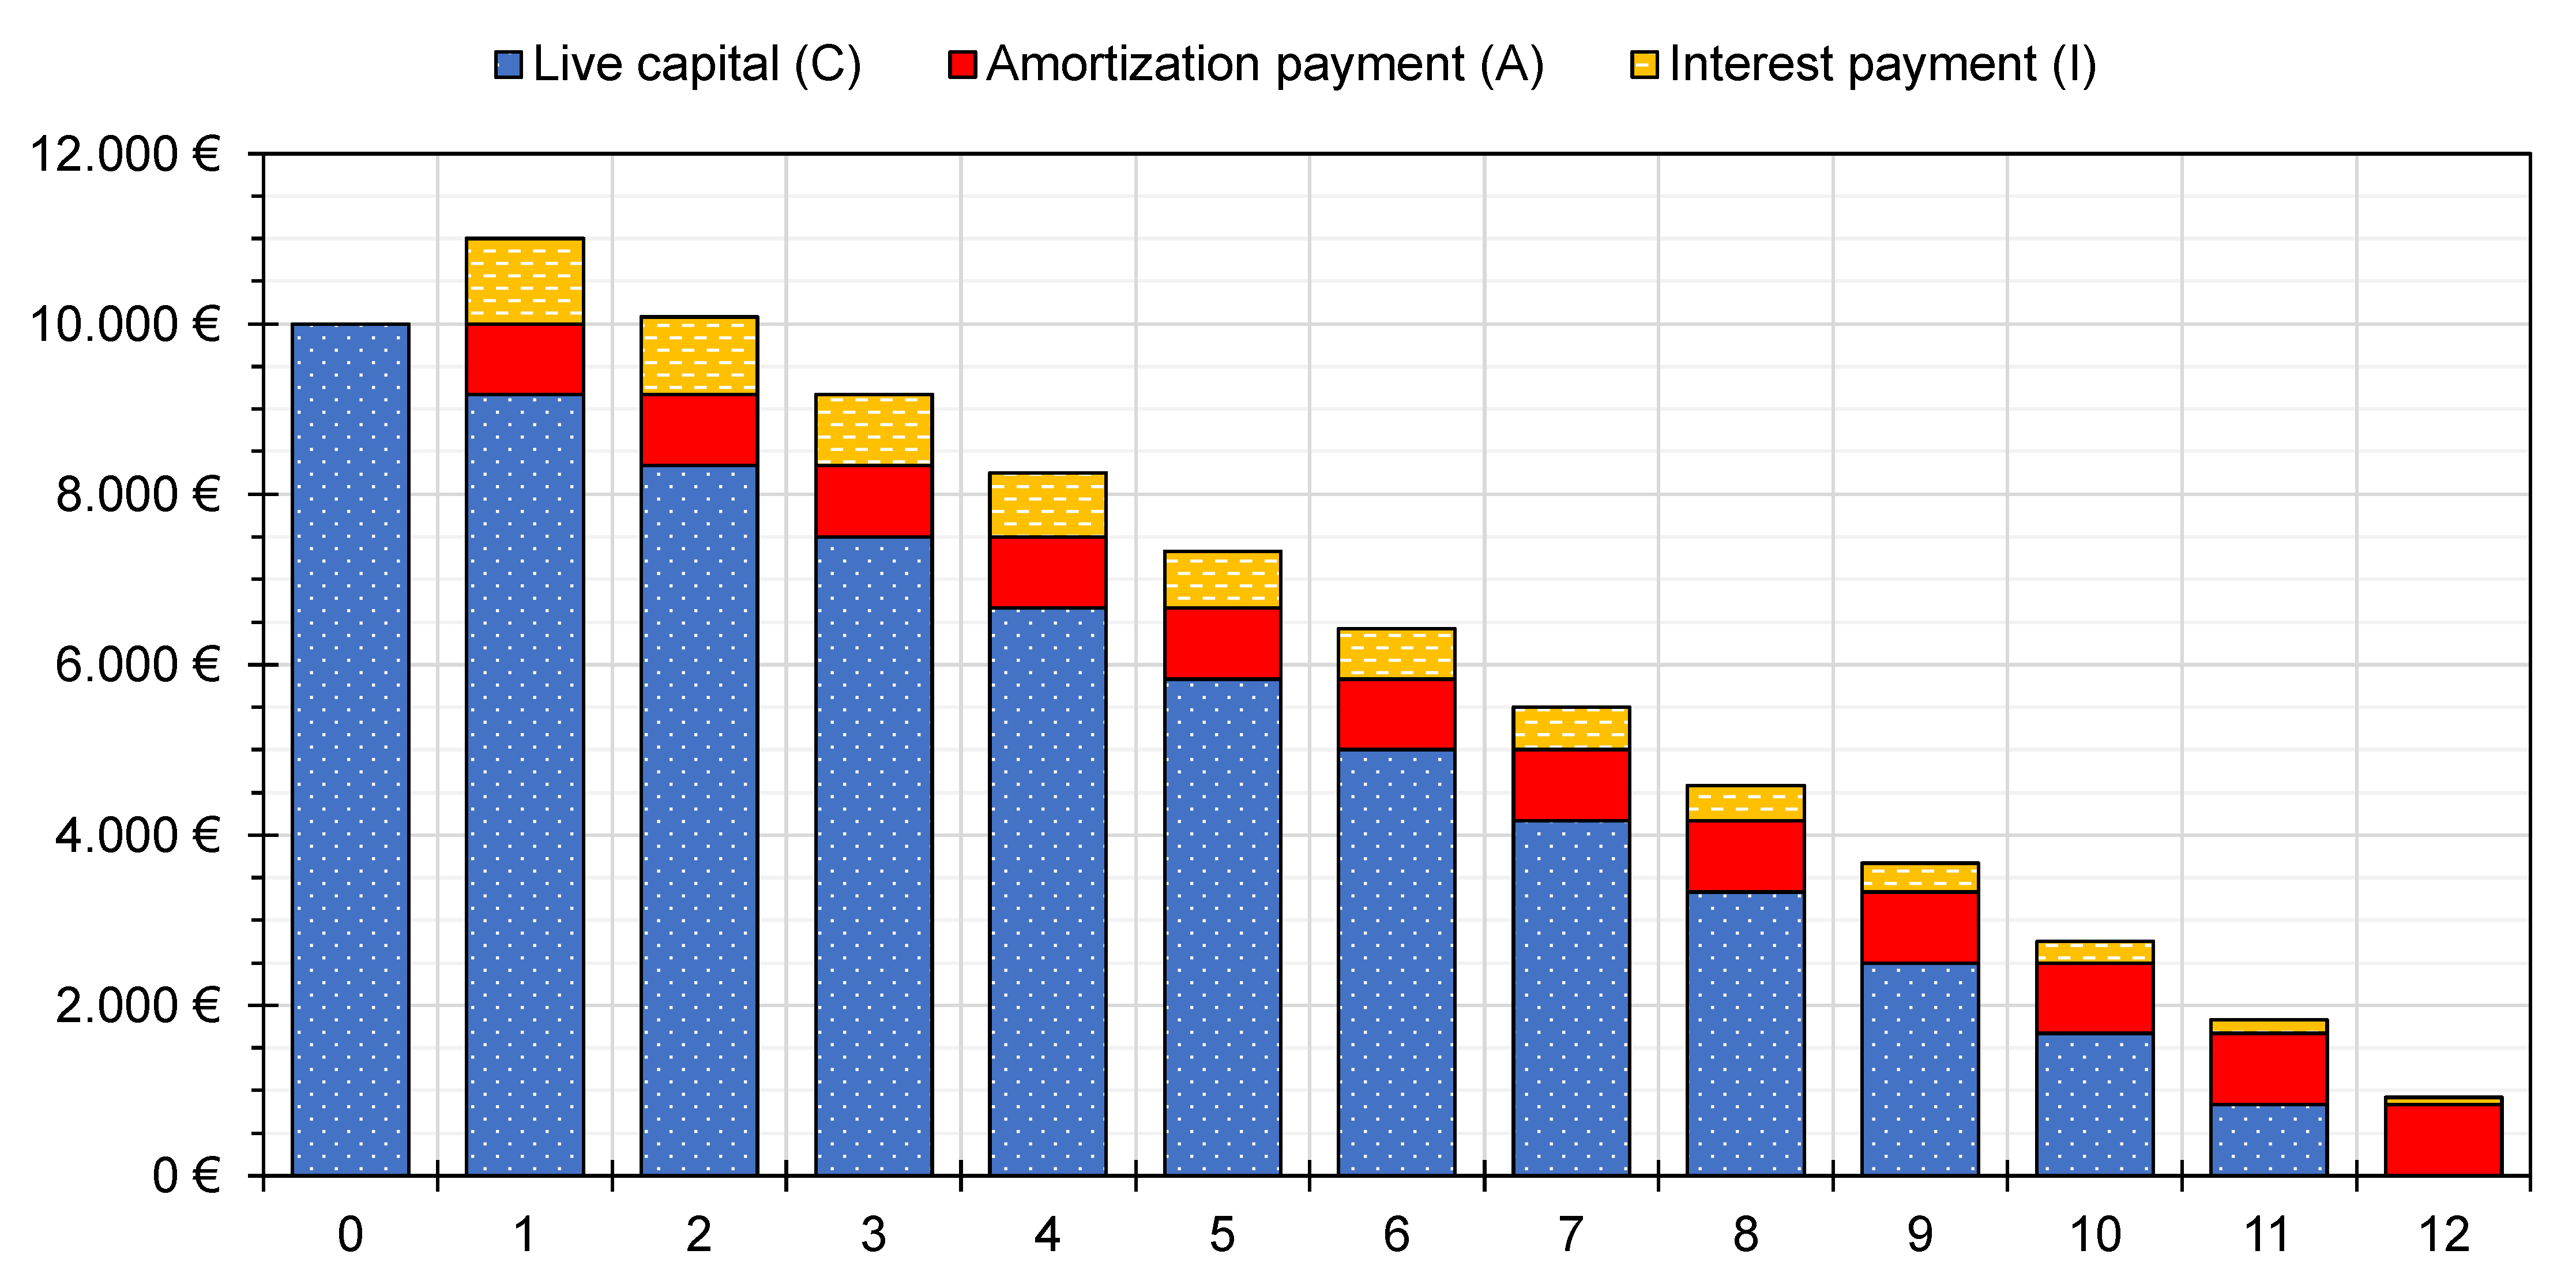
\includegraphics[width=11cm]{figures/italian-en.pdf}
	\end{center}
	
	\textbf{Loan with geometric progression terms}: amortization terms vary in geometric progression of factor $q$ (in this case, $q = 1.05$).
	
	\begin{center}
		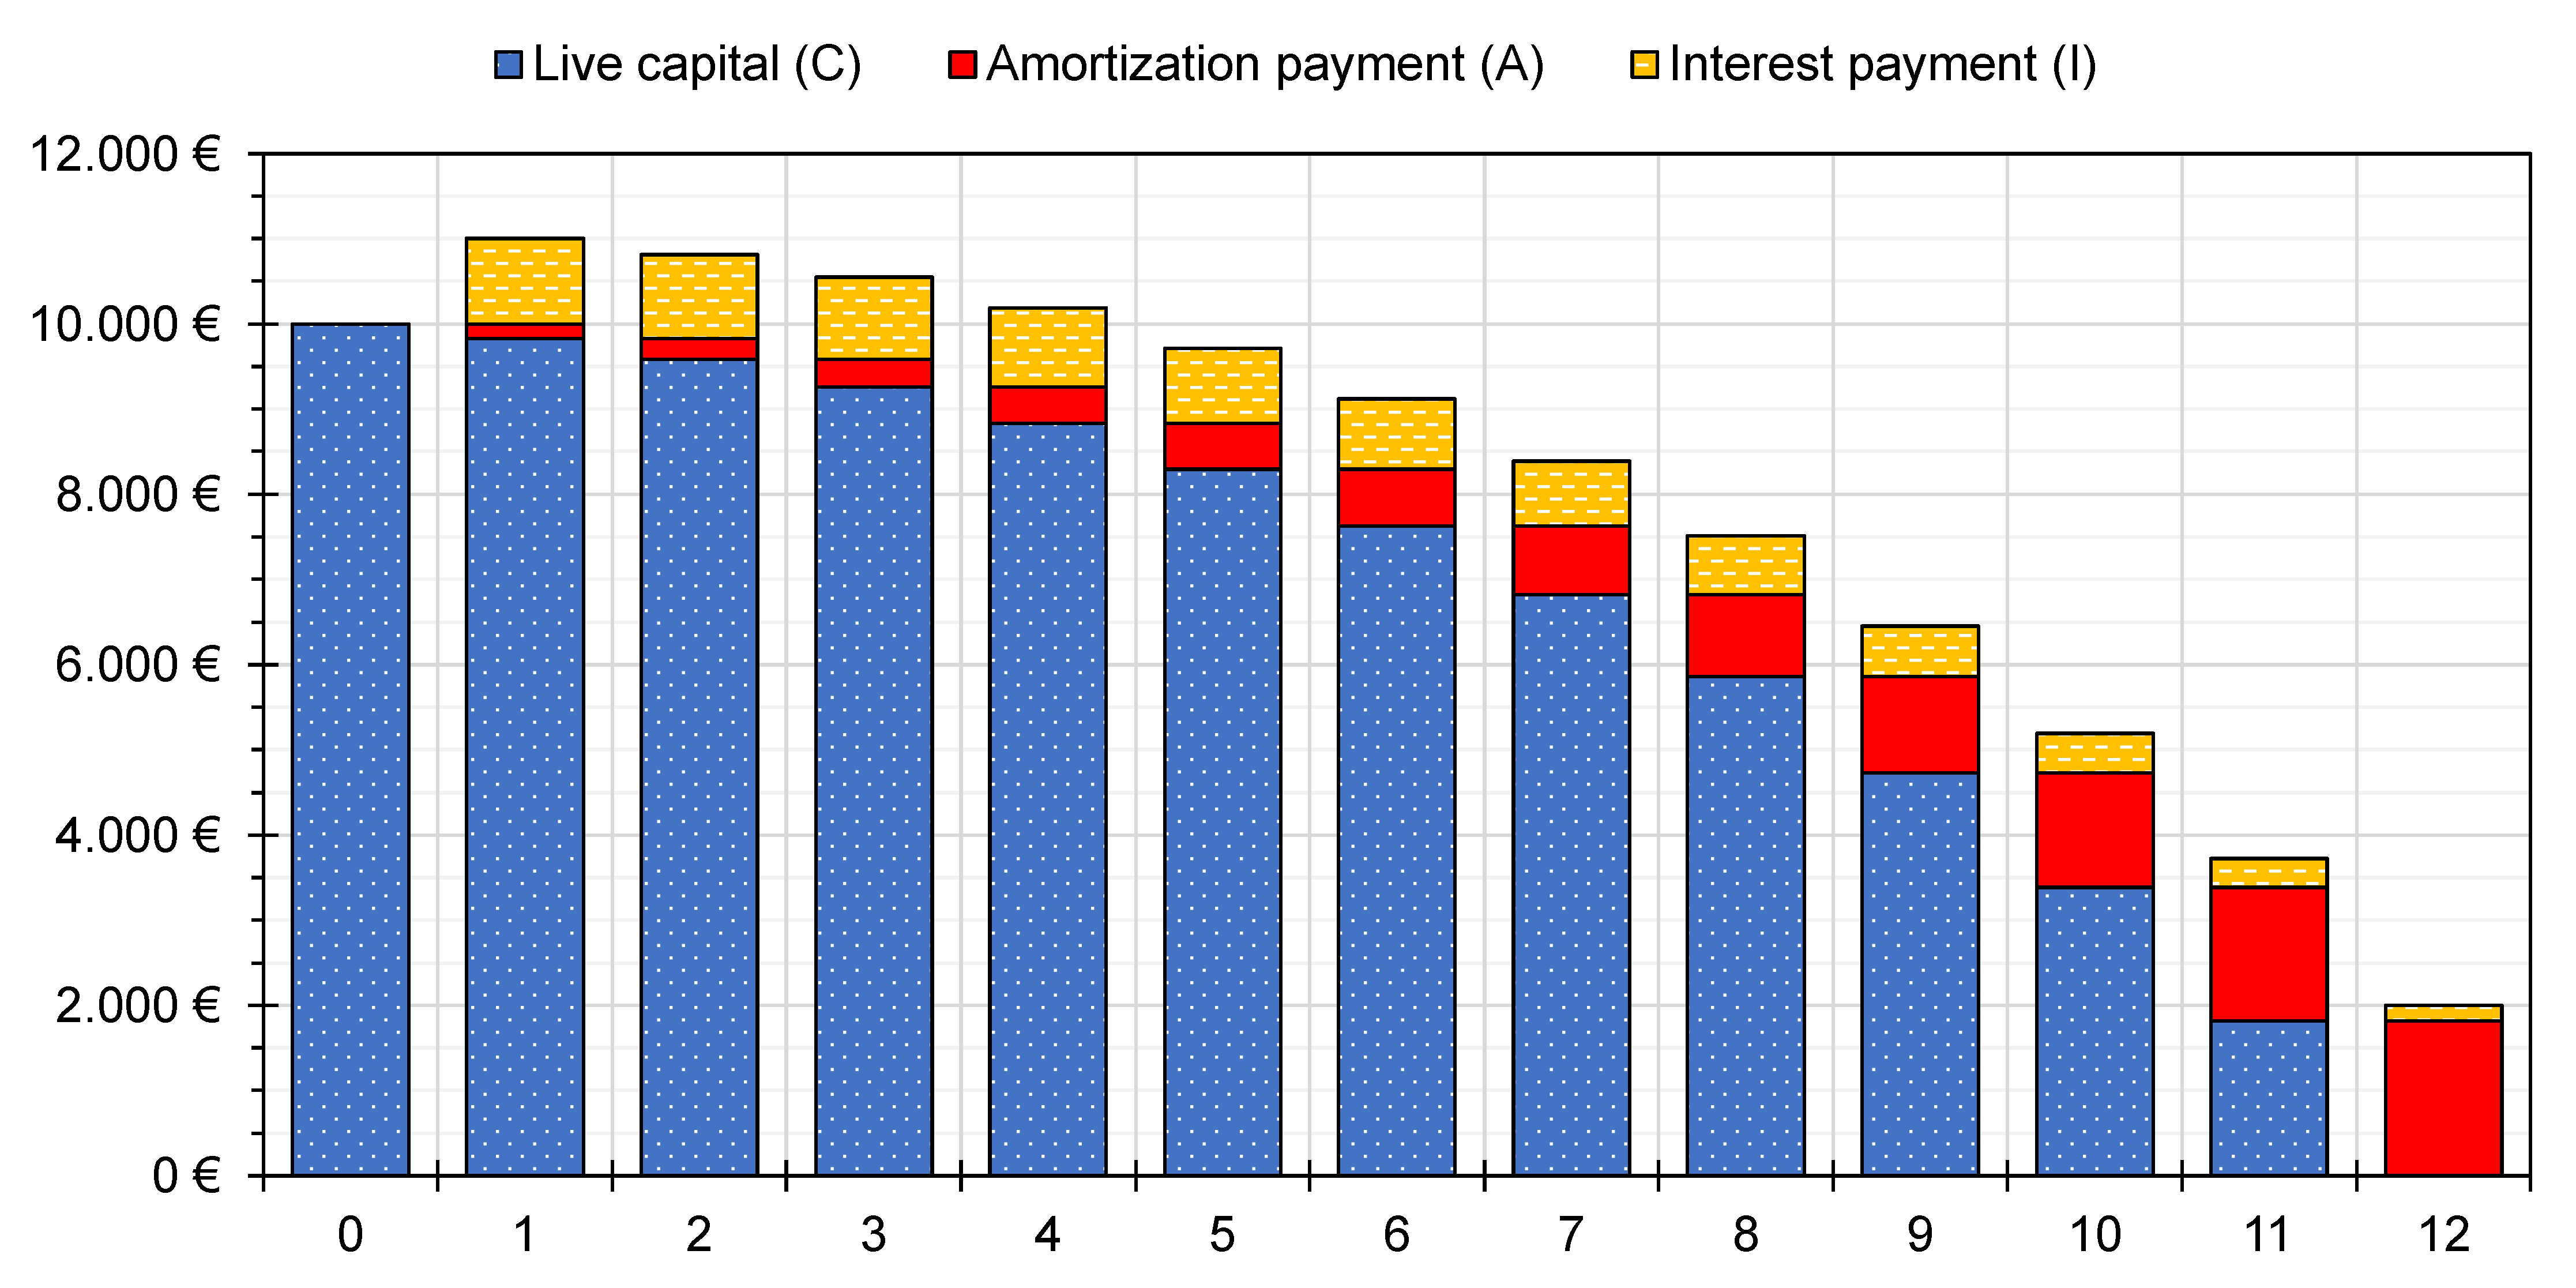
\includegraphics[width=11cm]{figures/geometric-en.pdf}
	\end{center}
	
\end{document}